\documentclass[../main.tex]{subfiles}
\begin{document}

\chapter{Integrative approaches for large-scale transcriptome-wide 
association studies, or: A test for significant \cis genetic correlation 
between expression and traits}
\labch{gusev2016}

\begin{external_abstract}{title=Abstract}
Many genetic variants influence complex traits by modulating gene 
expression, thus altering the abundance of one or multiple proteins. 
Here we introduce a powerful strategy that integrates gene expression 
measurements with summary association statistics from large-scale 
genome-wide association studies (GWAS) to identify genes whose 
cis-regulated expression is associated with complex traits. We leverage 
expression imputation from genetic data to perform a transcriptome-wide 
association study (TWAS) to identify significant expression-trait 
associations. We applied our approaches to expression data from blood 
and adipose tissue measured in \char`\~3,000 individuals overall. We 
imputed gene expression into GWAS data from over 900,000 phenotype 
measurements to identify 69 new genes significantly associated with 
obesity-related traits (BMI, lipids and height). Many of these genes are 
associated with relevant phenotypes in the Hybrid Mouse Diversity Panel. 
Our results showcase the power of integrating genotype, gene expression 
and phenotype to gain insights into the genetic basis of complex traits.
\end{external_abstract}

\section{Introduction}

The \textit{rationale} that lies behind the association of gene 
expression to phenotype is that many genetic variants influence traits 
by altering the regulation of the expression of some genes. Despite the 
strength of this argument, publications of studies in which both 
transcriptomic and phenotypic data are investigated simultaneously lag 
behind those of simple GWAS studies, for at least two reasons: first, 
although the cost of sequencing nucleic acids has been sharply 
decreasing for over a decade (\reffig{sequencingcost}), it can become 
quite an expensive technology if applied to cohorts of tens of thousand 
samples, such as those of a typical modern GWAS; secondly, every tissue 
shows a different pattern of expressed genes, and to choose the right 
tissue to analyse for each phenotype is not always a trivial matter.

\begin{marginfigure}[-4cm]
	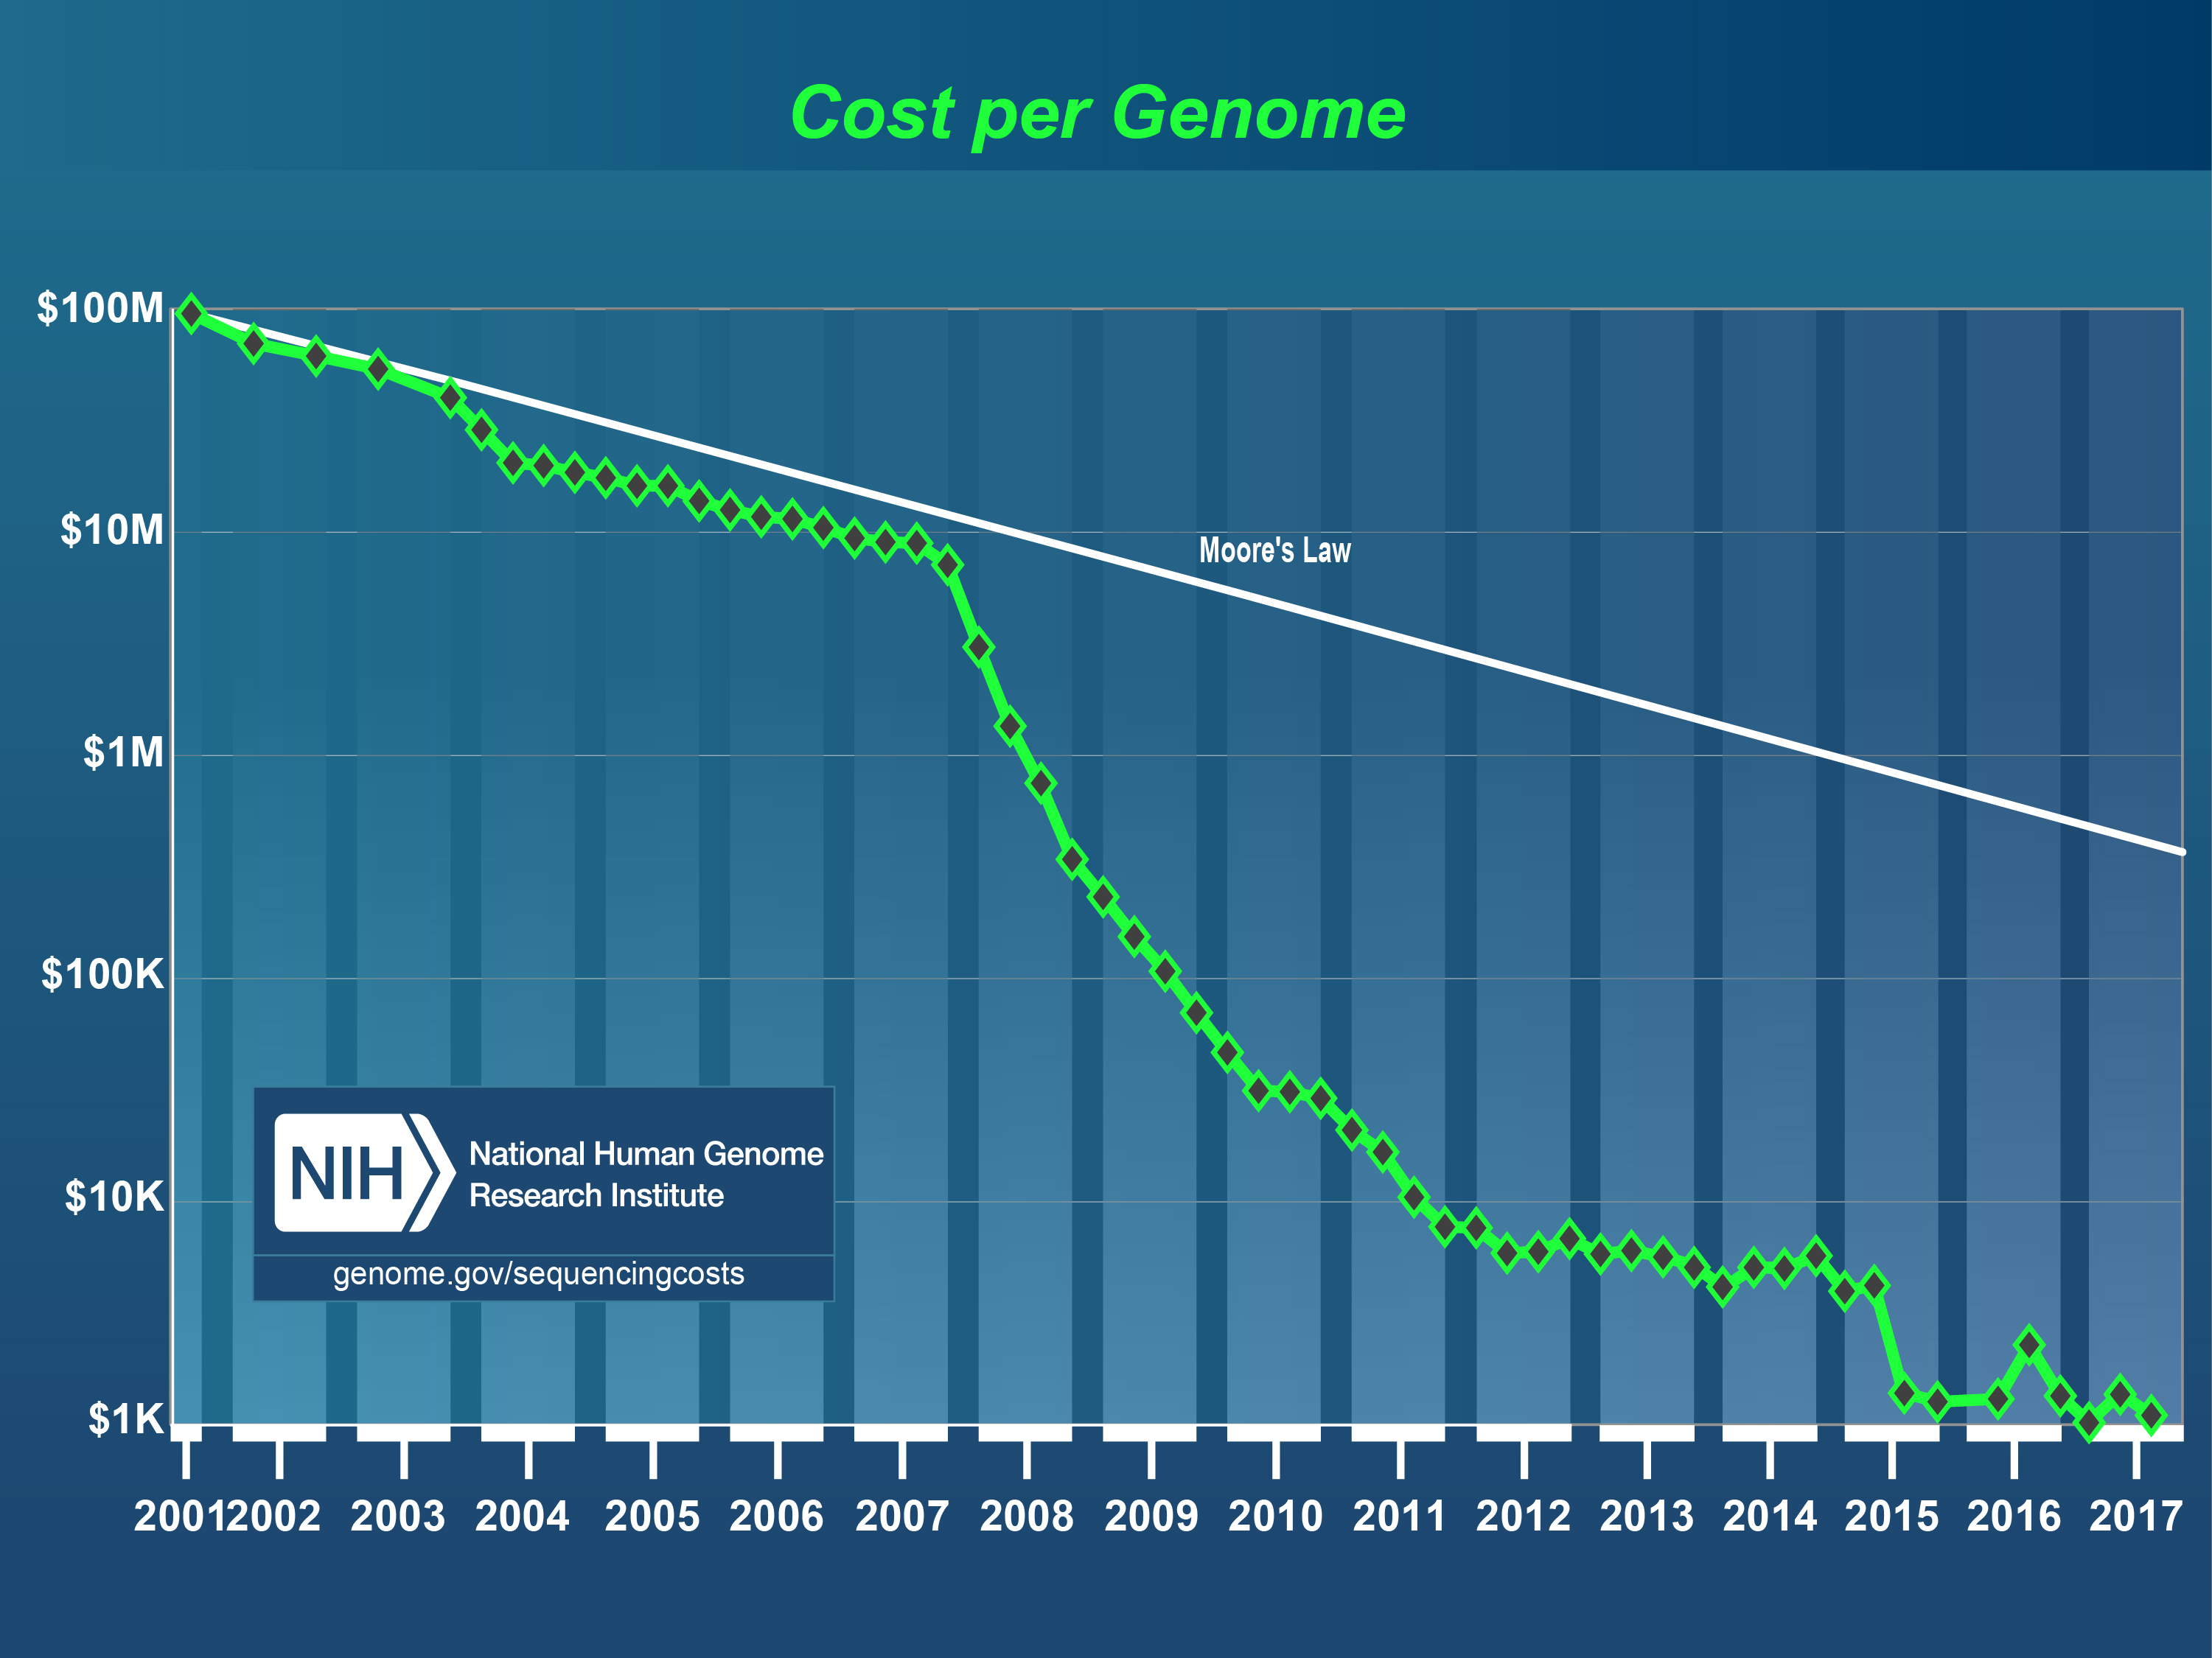
\includegraphics{sequencingcost}
	\caption[Sequencing cost over time]{The decrease in the cost of 
	genome sequencing; the same technology is used to sequence RNA. 
	\url{https://www.genome.gov/sequencingcosts/}}
	\labfig{sequencingcost}
\end{marginfigure}

In order to harness the plethora of data available from existing 
large-cohort GWAS studies, which, due to their great sample size, have 
the statistical power to find association even for rare and small-effect 
variants, many new methods are being developed. One of such methods is 
PrediXcan, with which we dealt in the previous section, but it is by no 
means the only one. In particular, in 2016 a new approach has been 
proposed which does not need individual-level data, but only summary 
association statistics\sidenote[][0cm]{By summary association statistics 
we mean, for instance, the effect size of all the SNPs} from a GWAS, 
which is an important advantage since, normally, only summary-level data 
is publicly available due to privacy concerns.

In essence, this approach is not different from PrediXcan: first, a 
linear regression model finds the correlation between each SNP and gene 
expression and accordingly assigns a weight to the SNP \todo{taking into 
account LD: gamazon used elastic net to prune correlated predictors}; 
next, the SNPs weights are used to impute the \cis genetic component of 
expression; finally, the imputed gene expression is tested for an 
association \todo{through correlation} with a complex trait.

\begin{figure}
	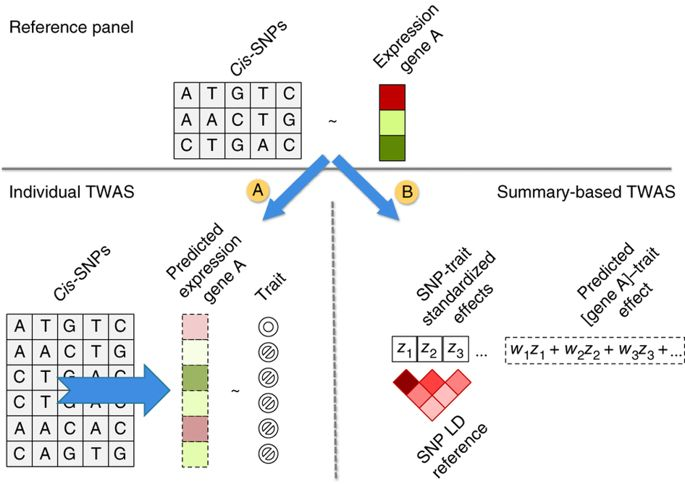
\includegraphics{gusev2016/1-TWAS_schematic}
	\caption{}
	\labfig{gusev2016/1}
\end{figure}

Nevertheless, there are some relevant points in this new method, 
relative to PrediXcan: its being based on summary association statistics 
greatly increases the effective sample size, because the method can in 
principle be applied to any GWA study; moreover, the authors emphasise 
the robustness of their approach, for its focus is on the genetic 
component of expression only, therefore it is guaranteed that the 
association between expression and trait is ultimately due to genetic 
factors.\todo{it doesn't mean it is robust}

Indeed, there are several ways in which genomic variation can be related 
to gene expression and phenotypic variation.\todo{approfondire}

\begin{marginfigure}[-2cm]
	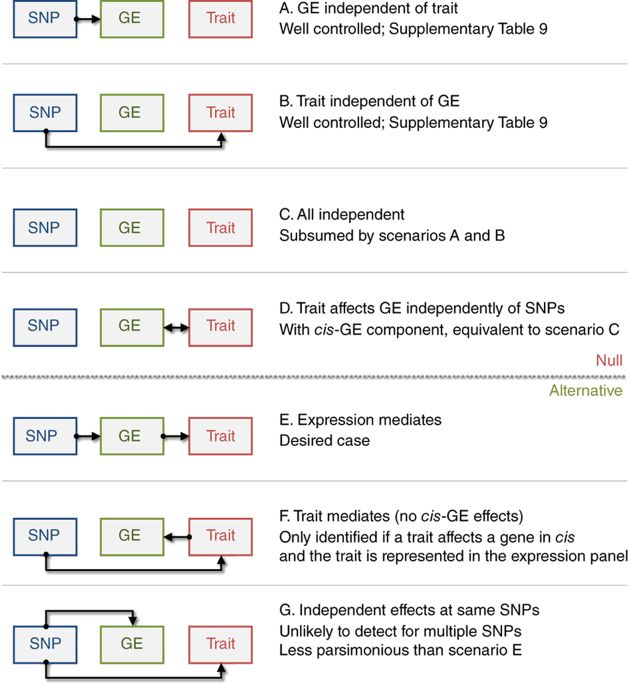
\includegraphics{gusev2016/2-causality_models}
	\caption{}
	\labfig{gusev2016/2}
\end{marginfigure}

\enquote{We applied our approaches to expression data from blood and 
adipose tissue measured in \char`\~3,000 individuals overall. Through 
extensive simulations and analyses of real data, we show that our 
proposed approach increases performance over standard GWAS and 
eQTL-guided GWAS. Furthermore, we reanalyzed a 2010 lipids GWAS17 to 
find 25 new expression-trait associations in those data. Among these 
associations, 19 of 25 contained genome-wide significant SNPs in the 
more recent and expanded lipids study5, thus showcasing the power of our 
approach to find robust associations. We imputed gene expression into 
GWAS data from over 900,000 phenotype measurements5,6,7 to identify 69 
new genes significantly associated with obesity-related traits (body 
mass index (BMI), lipids and height). Many of these genes were 
associated with relevant phenotypes in the Hybrid Mouse Diversity Panel 
(HMDP). Overall, our results showcase the power of integrating genotype, 
gene expression and phenotype to gain insights into the genetic basis of 
complex traits.}

\end{document}
